%% Contient le chapitre sur l'étude comparative entre les deux méthodes


\chapter{Etude comparative : Nuages de points et Mesh}

\section{Introduction}

\paragraph{•} Aujourd'hui, la modélisation d'objets 3D est devenu fondamentale dans de nombreux domaines tels que la robotique et les systèmes embarqués, l'animation, l'industrie ou encore les modèles à plus grande échelles permettant d'étudier le comportement d'un environnement. Or, la modélisation d'objets 3D est un problème complexe au centre de recherches. Les techniques les plus utilisées sont les nuages de points et les mesh 3D, aussi appelés maillage 3D. Nous allons dans un premier temps comparer ces deux méthodes de modélisation en les définissant et en explicitant leur principes, puis en étudiants leurs différentes limitations et enfin en analysant leurs domaines d'applications respectifs.



%%%%%%%%%%%%%%%%%%%%%%%%%%%%%%%%%%%%%%%%%%%%%%%%%%%%%%%%%%%%%
%% DEFINITION
%%%%%%%%%%%%%%%%%%%%%%%%%%%%%%%%%%%%%%%%%%%%%%%%%%%%%%%%%%%%%
\section{Définitions et propriétés}

\paragraph{•} Il convient dans un premier temps de définir ce qu'est un nuage de points et ce qu'est un mesh, aussi nommé maillage 3D. Nous allons voir dès la définition que ces deux objets sont très différents et ne peuvent être considérés de la même façon, ce qui va nous mener à une étude comparative de ces deux moyens de représentation d'objets 3D.

\subsubsection{Nuages de points}
\paragraph{•} Nous allons dans cette partie nous attarder sur la définition des nuages de points. Dans sa représentation la plus basique, un nuage de points est un type de données simple : dans la plupart des cas, un nuage de points n'est qu'une liste de points représentés par leur coordonnées 3D (i.e. une liste de coordonnées 3D).

On peut donc représenter un nuage de points comme l'ensemble :

\[ P = \{ x_{i} \in \Re^{3} \}_{i<N} \]

\newpage

Une représentation possible dans l'espace 3D :

\begin{figure}[h]
    \centering
    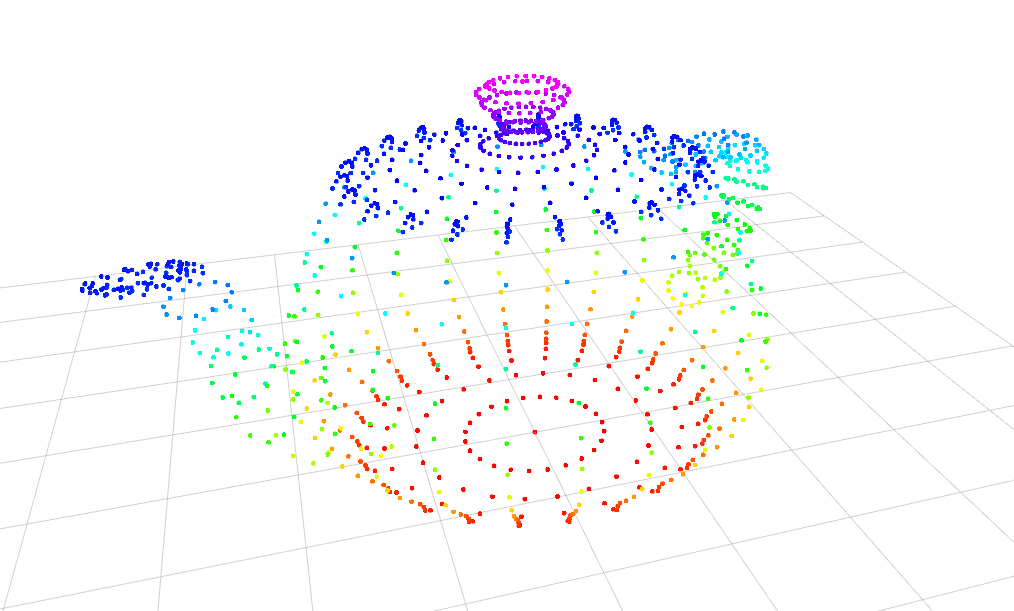
\includegraphics[width=0.50\textwidth]{headerimg}
    \caption{représentation d'un nuage de points dans l'espace}
    \label{fig:pointCloud1}
\end{figure}
\FloatBarrier

Dans notre cas ici $P$ est un ensemble de points sans lien logique et non ordonnés.
Mais notre vision actuelle est limitée par rapport à ce qui est possible de faire avec un nuage de points. En effet, rien ne nous empêche d'ajouter, en plus des informations spatiales (les coordonnées), d'autres informations, telles que la couleur des points ou encore la direction de la normale associée (très utile pour le passage de nuages de points vers mesh 3D par la méthode de reconstruction de poisson que nous verrons plus tard). Dans ce cas, le nuage de points obtenu est dit "augmenté" et on peut le représenter comme l'ensemble :

\[ P_{F} = \{ (x_{i}, f_{i}) | x_{i} \in \Re^{3}, f_{i} \in \Re^{D} \}_{i<N} \]

Ou $D$ est la dimension des informations liées à un point.
On utilise généralement des nuages de points colorés (c'est-à-dire avec des informations de dimension 3 : RGB) :

\begin{figure}[h]
    \centering
    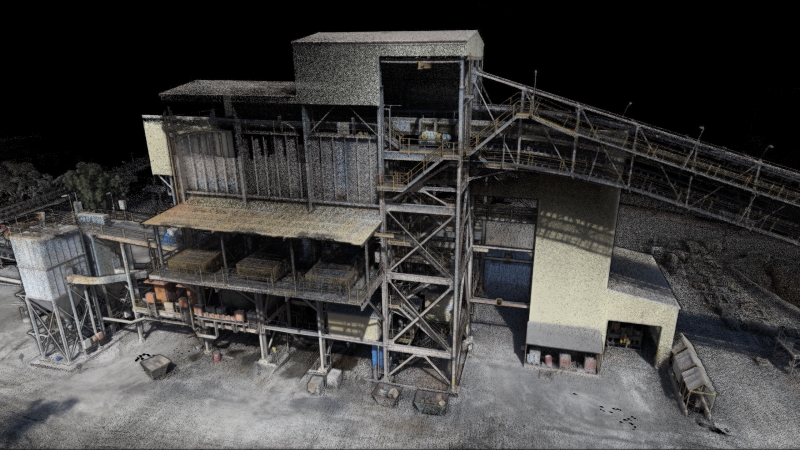
\includegraphics[width=0.50\textwidth]{ColoredPC}
    \caption{Nuage de points colorés}
    \label{fig:pointCloud2}
\end{figure}
\FloatBarrier


\newpage
En récapitulatif :

\begin{figure}[h]
    \subfloat[Espace vide]{
        \begin{minipage}[c][1\width]{
            0.3\textwidth}
            \centering
            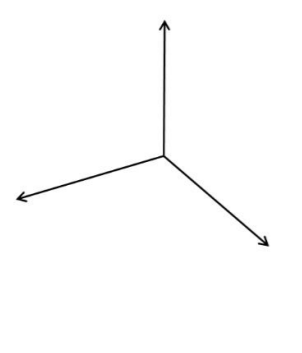
\includegraphics[width=1\textwidth]{Capture3}
        \end{minipage}}
    \hfill
    \subfloat[Ensemble $P$]{
        \begin{minipage}[c][1\width]{
            0.3\textwidth}
            \centering
            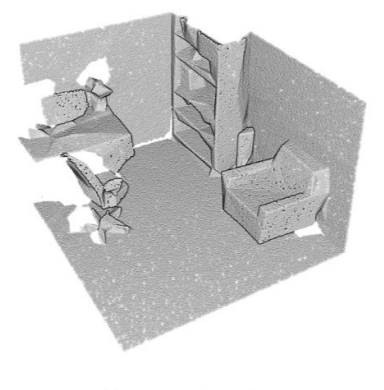
\includegraphics[width=1.1\textwidth]{Capture1}
        \end{minipage}}
    \hfill
    \subfloat[Ensemble $P_{F}$]{
        \begin{minipage}[c][1\width]{
            0.3\textwidth}
            \centering
            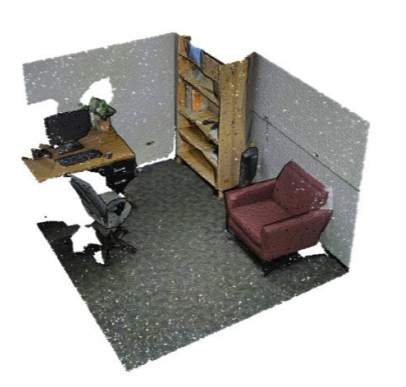
\includegraphics[width=1.2\textwidth]{capture2}
        \end{minipage}}
    \caption{}
    \label{fig:figure1}
\end{figure}
\FloatBarrier

les nuages de points obtenus sont donc une représentation discrète et non-ordonnée de points de l'espace.

\FloatBarrier
\subsubsection{Maillages 3D}
\paragraph{•} Nous allons maintenant nous attarder sur la définition des maillages 3D, aussi appelés mesh 3D. Un mesh 3D, de par sa plus grande complexité par rapport aux nuages de points, peut être défini de plusieurs façons. Nous allons ici nous focaliser sur sa version la plus commune.
\paragraph{•} Un modèle 3D représente une collection de points (appelés vertex) dans l'espace, connectés par des liens géométriques. On peut par exemple citer les liens sous forme de triangles, lignes ou surfaces.
Ce type de représentation permet donc à l'inverse des nuages de points d'avoir un ensemble de points ordonnés et donc liés les uns avec les autres pour former une forme géométrique. Il est alors possible d'en extraire des informations plus riches que les nuages de points. On peut par exemple obtenir la surface du modèle ou encore son orientation.



\begin{figure}[h]
    \centering
    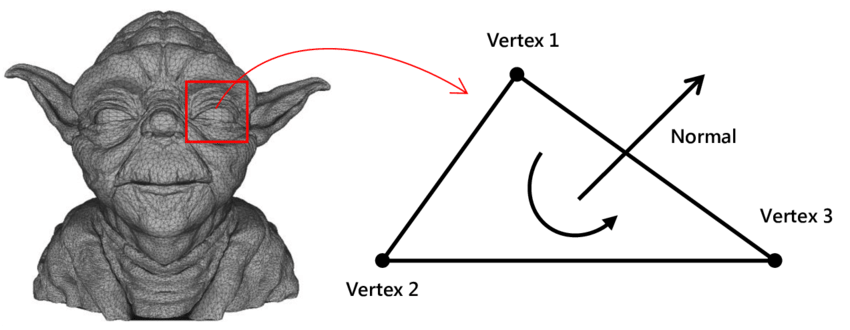
\includegraphics[width=0.50\textwidth]{Structure-of-a-3D-triangle-mesh}
    \caption{Exemple de mesh 3D}
    \label{fig:Structure-of-a-3D-triangle-mesh}
\end{figure}
\FloatBarrier



On ne donne pas de définition mathématique des maillages 3D (possible mais cela sort du contexte de ce rapport). En effet, pour avoir une définition exacte il faut préciser le type de maillage : mesh structuré, mesh structuré par blocs ou mesh non-structuré.
Nous nous contenterons donc ici d'une approche plus générale.

Ainsi, les nuages de points peuvent être vus comme une vision discrète non-ordonnée du monde 3D alors que les maillages 3D nous donne une vison continue ordonnée et donc plus riche.
\FloatBarrier


%%%%%%%%%%%%%%%%%%%%%%%%%%%%%%%%%%%%%%%%%%%%%%%%%%%%%%%%%%%%%
%% METHODES D'ACQUISITION
%%%%%%%%%%%%%%%%%%%%%%%%%%%%%%%%%%%%%%%%%%%%%%%%%%%%%%%%%%%%%
\section{Méthodes d'acquisition}
Nous allons maintenant étudier les différentes façons dont il est possible d'obtenir une représentation 3D du monde réel sous forme de nuages de points ou de mesh 3D. Nous allons pour ce faire présenter 3 catégories de méthodes d'acquisition différentes : la première qui permet l'acquisition de nuages de points (scanner laser), la deuxième permettant d'obtenir des volumes 3D sous forme de mesh (caméra avec vison de profondeur, IRM...) et finalement des méthodes dites hybrides qui permettent l'obtention de mesh et de nuages de points (photogrammétrie, stéréographie...).

%% Mettre cette étape en conclusion
Il est important de noter que l'obtention de mesh 3D est très difficile, car il demande une lecture continue de l'espace 3D. Cela est souvent uniquement possible dans un espace restreint et durant un temps limité. Par opposition, l'obtention de nuages de points est beaucoup plus simple et permet une reconstruction du mesh 3D. C'est souvent cette dernière méthode qui est utilisée lors de la construction de mesh 3D, car elle est plus simple à mettre en place.
\subsection{Acquisition de nuages de points}
\subsubsection{Principe}
\paragraph{•} La méthode d'acquisition la plus représentative lorsque l'on parle de nuages de points et la plus répandue aujourd'hui est celle dite des scanner laser. Dans ce cadre les LiDAR (Light Detection And Ranging) sont les capteurs les plus privilégiés. Bien que les LiDAR peuvent être fondés sur différentes technologies, ils partagent le même principe : il s'agit d'un "Radar électromagnétique", un émetteur émet une pulsation électromagnétique qui se réfléchie sur un sujet, pour ensuite être captée par un récepteur. La durée entre l'émission et la réception de l'impulsion permet de déterminer la distance à l'objet.

\begin{figure}[h]
    \centering
    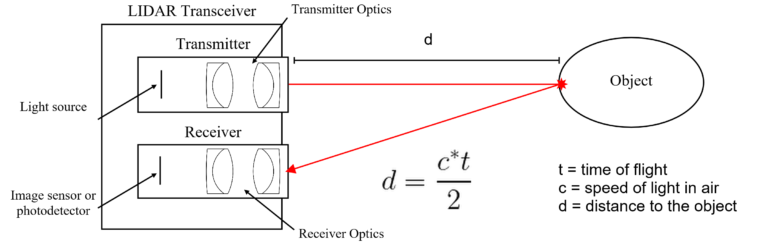
\includegraphics[width=0.50\textwidth]{lidarWorks}
    \caption{Principe de fonctionnement d'un LiDAR}
    \label{fig:lidarWork}
\end{figure}
\FloatBarrier
Cette méthode permet alors d'obtenir des nuages de points de très grande qualité, ci-dessous quelques exemples :

\begin{figure}[h]
    \centering
    \subfloat[ Vue dans l'axe du LiDAR]{{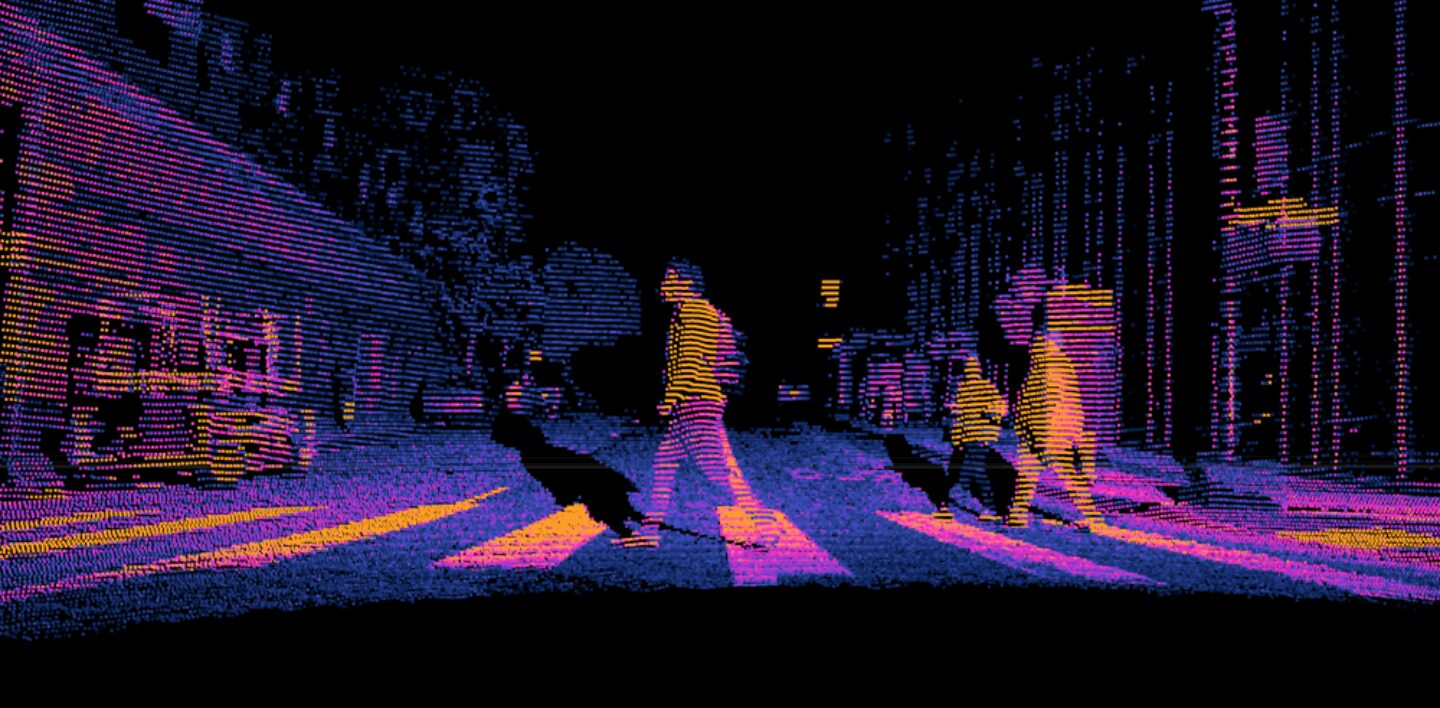
\includegraphics[width=6cm]{FrontViewLIdar} }}
    \qquad
    \subfloat[ Vue globale de la carte 3D]{{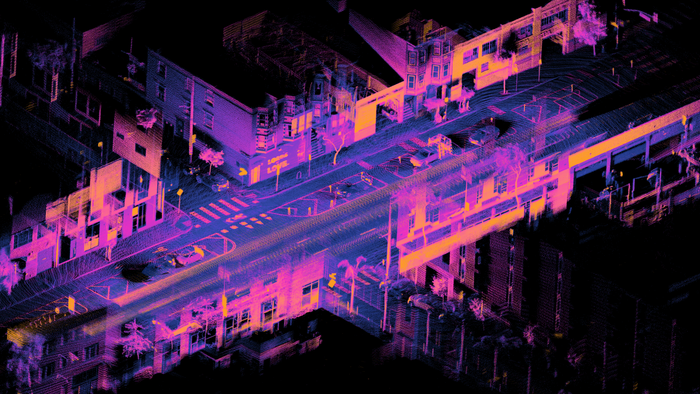
\includegraphics[width=5cm]{lidarExamplePC} }}
    \caption{Nuages de points obtenus d'un LiDAR Ouster OS1-128}
    \label{fig:PCLidar}
\end{figure}
\FloatBarrier

Nous verrons ensuite comment ces nuages de points peuvent être traités pour permettre la génération de maillages 3D. Cette méthode peut être appliquée ici pour permettre l'obtention de maillage 3D à partir des données LiDAR.

\subsubsection{Capteurs}
Le LiDAR nécessite des équipements spécifiques et coûteux. Cependant, leur coût de production diminue avec la démocratisation de la technologie (avec l'intégration de scanner LiDAR dans plusieurs smartphones flagships par exemple).
\begin{figure}[h]
    \centering
    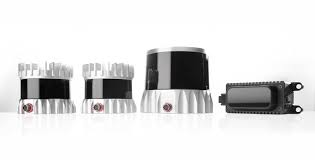
\includegraphics[width=0.5\textwidth]{ousterLidars}
    \caption{Gamme de capteur LiDAR Ouster}
    \label{fig:ousterLidars}
\end{figure}
\FloatBarrier


\subsection{Acquisition de maillages 3D}
\subsubsection{Principe}
\paragraph{•} En pratique, l'acquisition des maillages 3D est beaucoup plus complexe que celle des nuages de points. En effet les maillages 3D comportent une information continue et précise de la géométrie 3D. En d'autre termes, une représentation exacte de la surface du modèle. Or être capable de précisément déterminer le volume et la surface de l’environnement réel nécessite des technologies très complexes.
On peut, néanmoins, citer certaines de ces technologies et leurs limitations. On a notamment les scaneurs IRM qui permettent d'obtenir une information volumétrique (à partir de plusieurs tranches mises bout à bout et interpolées) mais ne sont opérationnels que sur de petits volumes.
\newline
D'autre part avec l’apparition de méthodes plus modernes, qui utilisent l'intelligence artificielle, on peut aujourd’hui reconstruire un modèle 3D à partir d'une simple information 2D. Nous allons nous attarder ici à l'état de l'art actuel, pifuhd développé par facebook reasearch lab \cite{saito2020pifuhd}.
La solution proposée permet de générer un mesh 3D à partir d'une image 2D d'une personne.

\begin{figure}[h]
    \centering
    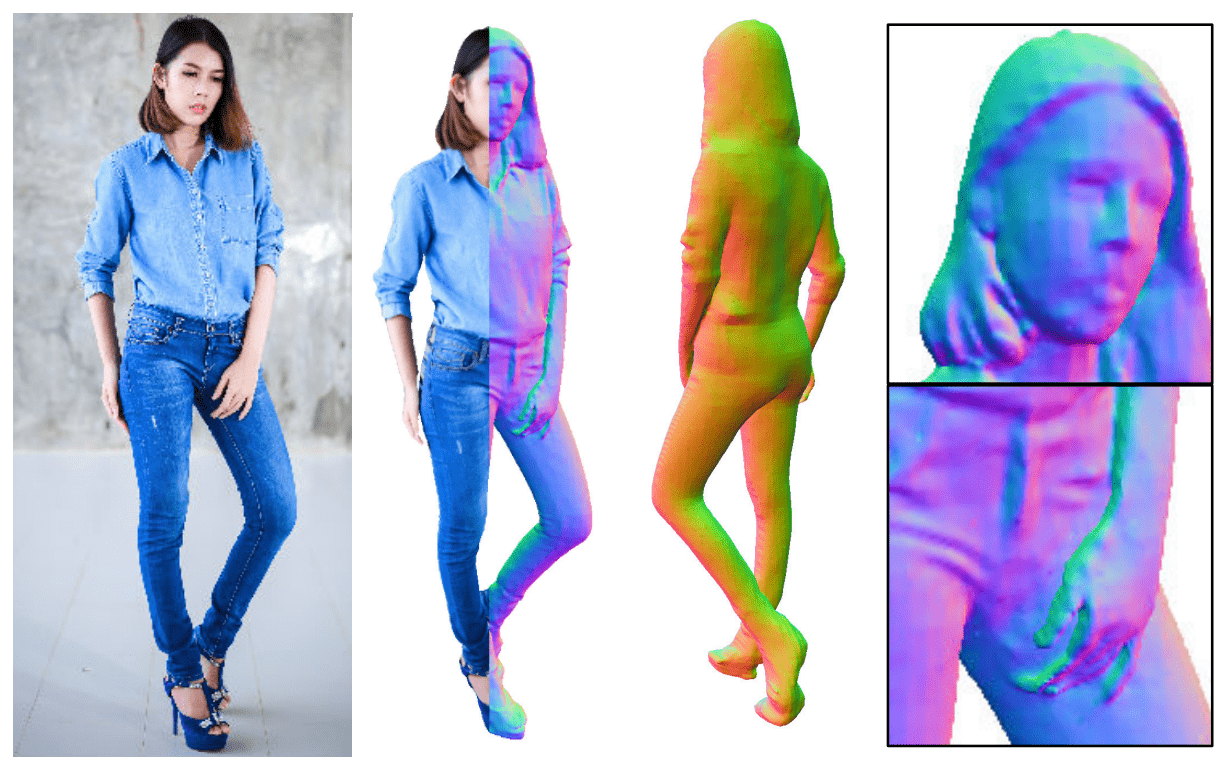
\includegraphics[width=0.50\textwidth]{pifuhd}
    \caption{Etapes de génération de pifuhd}
    \label{fig:pifuhd}
\end{figure}
\FloatBarrier

Le logiciel utilise une méthode d'optimisation implicite à partir d'une analyse de l'image 2D à plusieurs niveaux (Multi-Level Pixel-Aligned Implicit Function optimization). On peut se représenter cette méthode comme une méthode utilisant des templates. En effet, ici, nous partons d'un modèle 3D universel représentant une personne. Puis, On déforme ce modèle pour le faire correspondre aux proportions de l'image.

\begin{figure}[h]
    \centering
    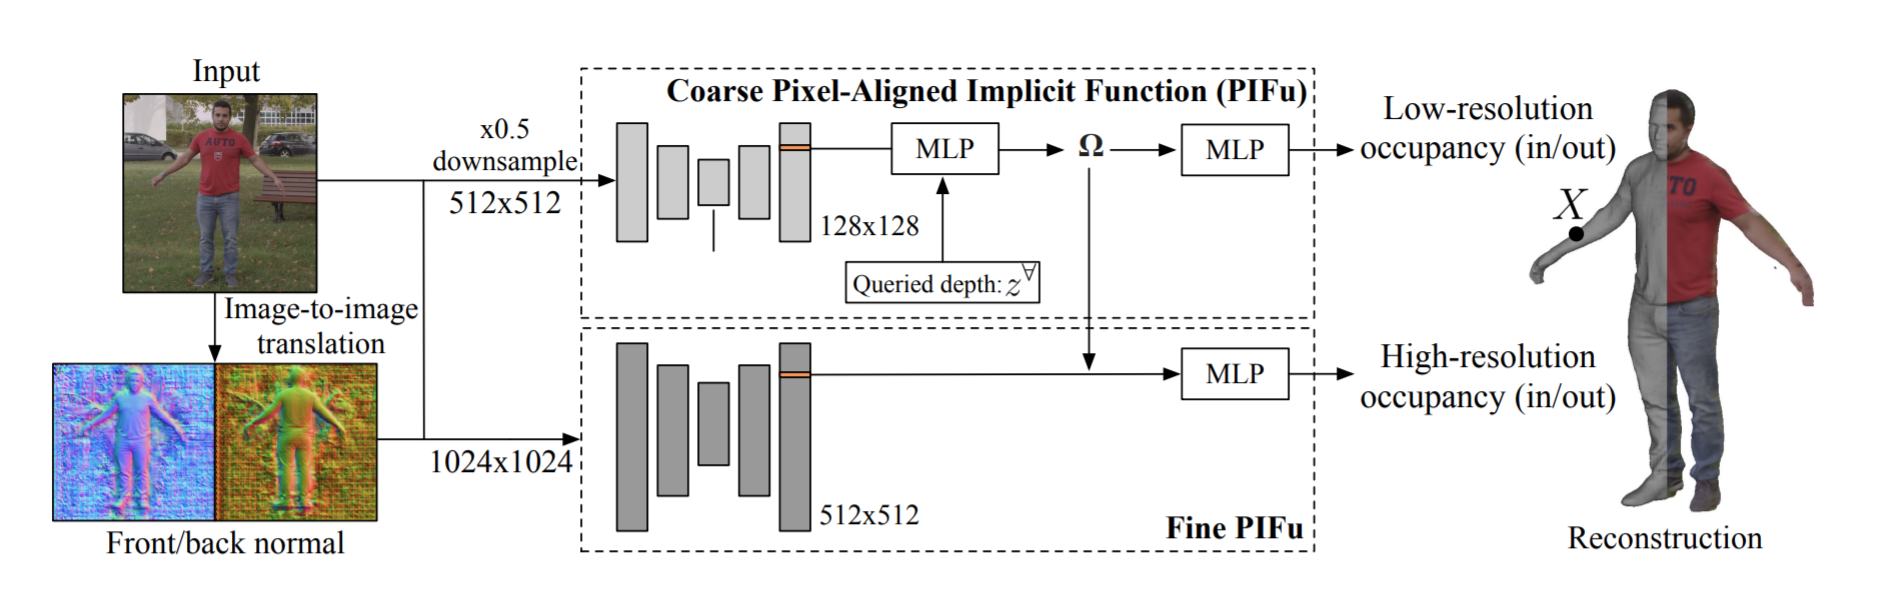
\includegraphics[width=0.8\textwidth]{pifuhdWork}
    \caption{Fonctionnement interne de pifuhd}
    \label{fig:pifuhdWork}
\end{figure}
\FloatBarrier

Ces méthodes de génération de modèles 3D à partir d'une information de dimension inférieure (i.e. image 2D) sont vouées à être de plus en plus utilisées. En effet elles permettent l'obtention d'un modèle 3D de meilleure qualité et avec une complexité moindre qu'en passant par la génération d'un nuage de point. Ce genre de méthode, bien qu'ici réduite à la simple modélisation de personnes, à été aussi étendue à d'autre domaines, comme l'imagerie médicale ou la génération de surfaces topographiques (DSM : Digital elevation terrains)\cite{DSM}.


\subsection{Méthodes hybrides}

\paragraph{•} Pour le moment nous avons vu comment obtenir des nuages de points et des maillages 3D directement et indépendamment les un des autres. Mais dans la pratique, il n'est pas rare de passer par des méthodes hybrides où l'on génère en premier lieu un nuage de points, puis, à partir de ce nuage de points, on génère le maillage 3D à l'aide de différentes méthodes de reconstruction. Il existe deux méthodes très largement utilisées :

\subsubsection{Photogrammétrie} La photogrammétrie  consiste a utiliser des collections de prises de vue 2D d'un sujet pour en recréer une représentation tridimensionnelle. La Photogrammétrie se fait en trois grandes étapes : il faut d'abord positionner les photos prises dans l'espace afin d'obtenir les positions et orientations du capteur lors de la prise, on appelle cette étape bundle adjustment; puis vient l'étape de projection d'un ensemble de points (appelé features) dans l'espace. C'est avec cet ensemble de points projetés que l'on peut finalement densifier le nuage de points jusqu'à obtenir un nuage de point dense). Ces méthodes sont appelées sfm (structure from motion) \cite{orb} \cite{mvg} :

\begin{figure}[h]
    \centering
    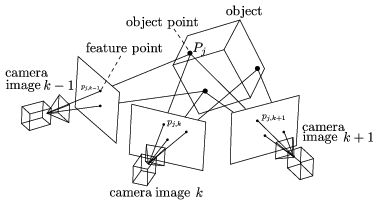
\includegraphics[width=0.4\textwidth]{sfm}
    \caption{Structure From Motion}
    \label{fig:sfm}
\end{figure}
\FloatBarrier

On peut alors obtenir sous forme d'un nuage de point dense la représentation de l'environnement :

\begin{figure}[h]
    \centering
    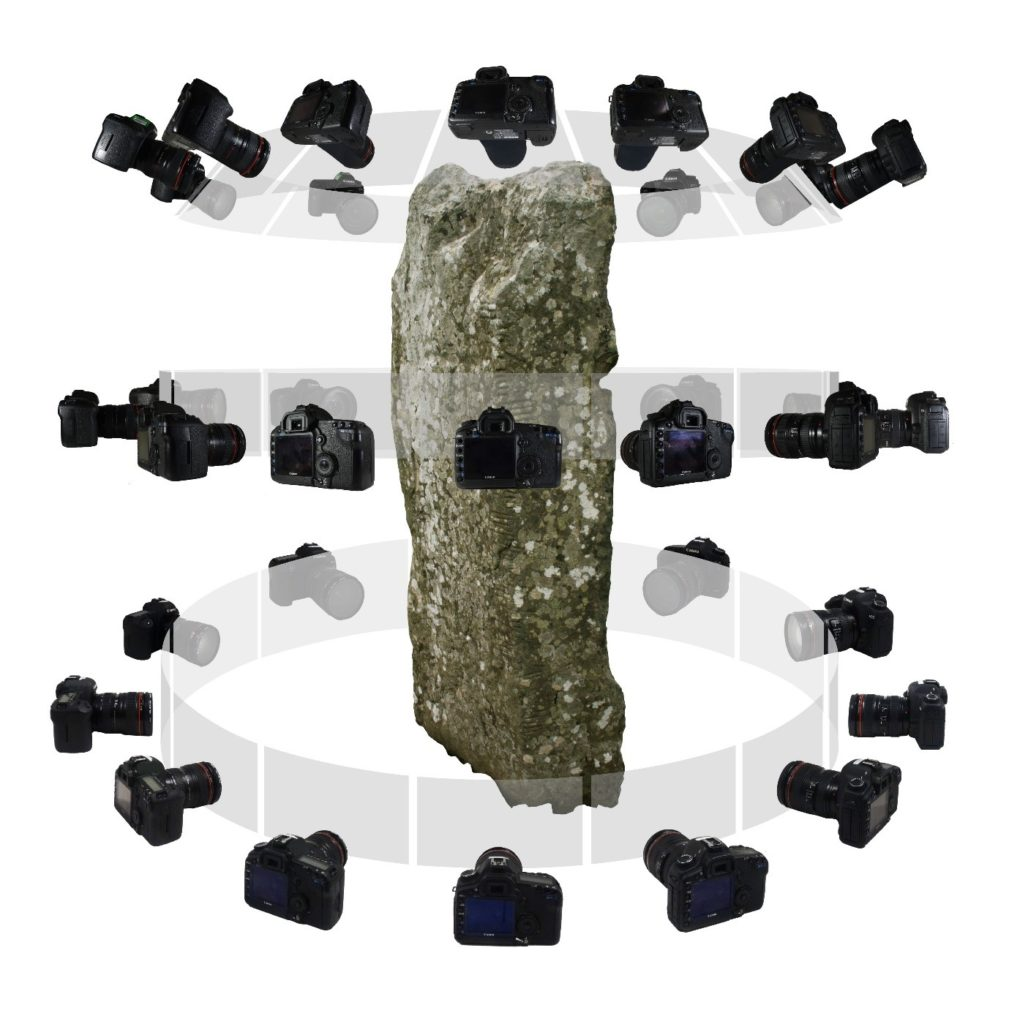
\includegraphics[width=0.3\textwidth]{photog}
    \caption{Nuage de points reconstruit à partir des images}
    \label{fig:photog}
\end{figure}
\FloatBarrier


Il est alors possible à partir de ce nuage de point d'obtenir un maillage 3D. Il existe plusieurs méthodes le permettant. La plus connue est celle dite de reconstruction de poisson \cite{poisson}, mais elle demande la connaissance des normales associées à chaque point (ce qui ajoute une étape de calcul). Nous allons donc ici présenter une méthode plus générale : Advancing Front Surface Reconstruction \cite{dddddd}. En effet cette méthode, avec un peu de pré et post-traitement, permet l'obtention d'un maillage 3D de très bonne qualité à partir d'un nuage de points dense.

\begin{figure}[h]
    \centering
    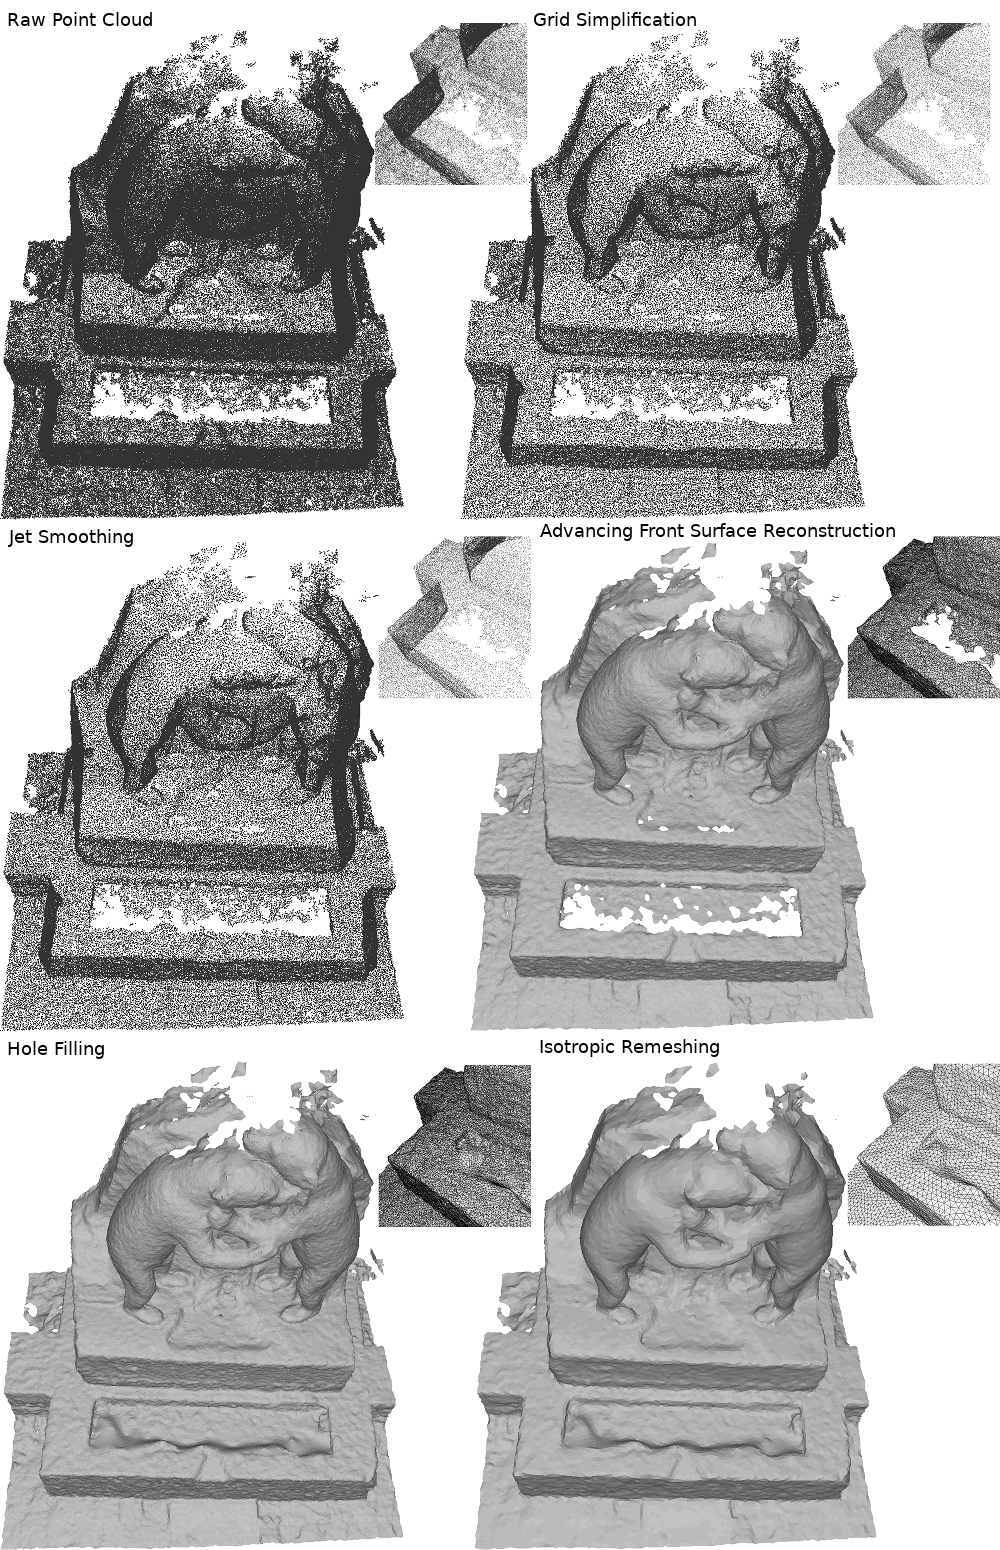
\includegraphics[width=0.35\textwidth]{reconstruction}
    \caption{Exemple de reconstruction utilisant cette méthode à l'aide de CGAL}
    \label{fig:photog}
\end{figure}
\FloatBarrier


\subsubsection{Depth map} 
De plus, nous pouvons présenter les caméras à profondeur de champ (depth cameras). Elles ne permettent pas directement d'obtenir un mesh 3D, mais elles fournissent une surface pouvant être utilisée pour la reconstruction du mesh 3D. Similaire à la photogrammétrie, elles sont constituées de deux cameras qui permettent d'obtenir une vision stéréoscopique, on peut alors extraire une information de profondeur sous forme de nuage de points, puis d'image 2D associant à chaque pixel sa profondeur relative par rapport au capteur, qui peut être utilisé par la suite pour générer un mesh 3D de la surface située en face de la caméra (Stéréoscopie) \cite{book1} .

\begin{figure}[h]
    \centering
    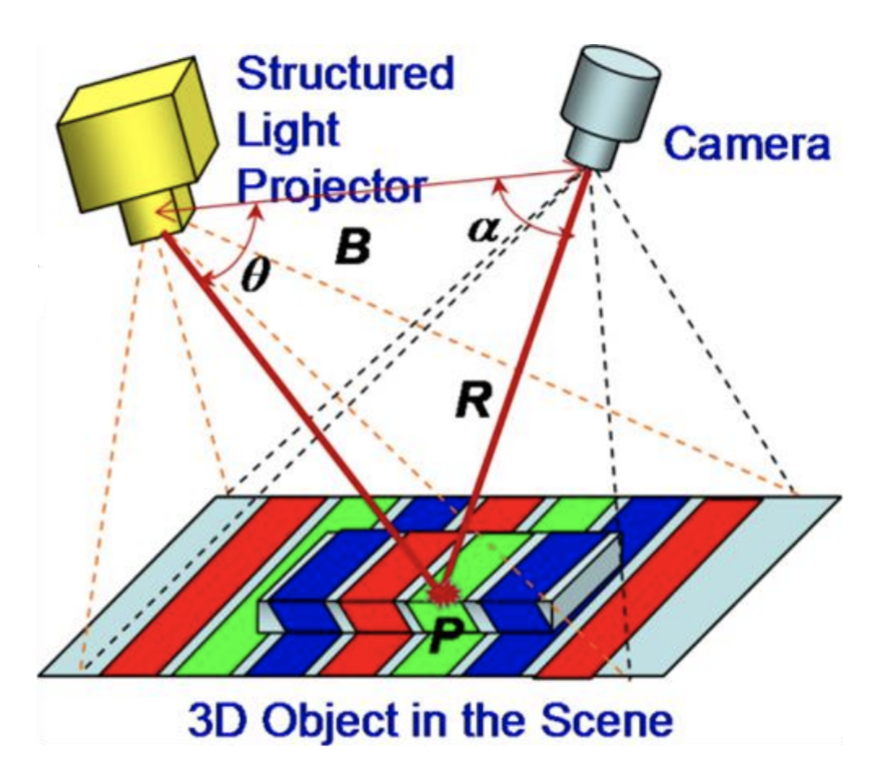
\includegraphics[width=0.4\textwidth]{stt}
    \caption{Fonctionnement de la Stéréoscopie}
    \label{fig:pifuhdWork2}
\end{figure}
\FloatBarrier

On obtient alors une carte de la profondeur vu par la caméra (depth map) :

\begin{figure}[h]
    \centering
    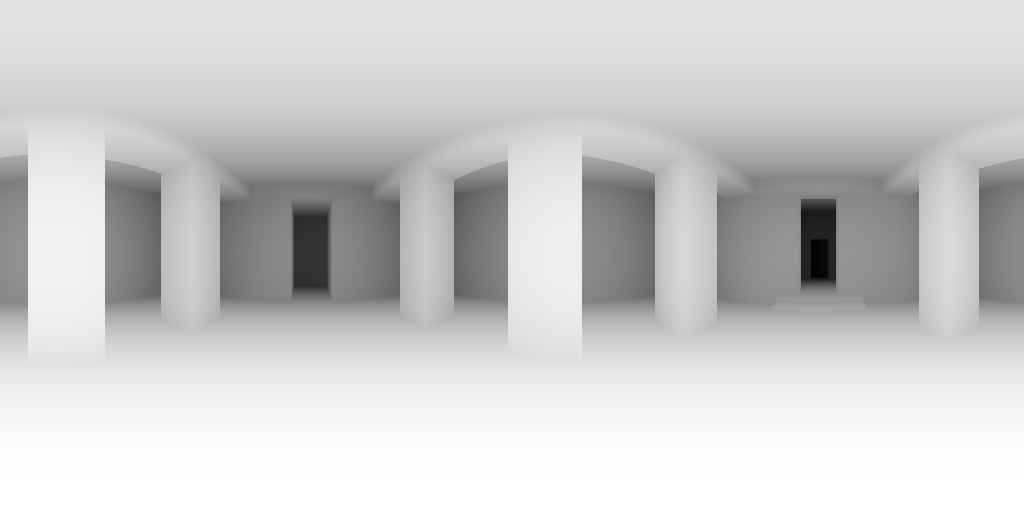
\includegraphics[width=0.8\textwidth]{depthmap}
    \caption{image obtenue, noir = loin, blanc = près}
    \label{fig:pifuhdWork3}
\end{figure}
\FloatBarrier

Pour obtenir un modèle 3D fermé représentatif, il faut alors se déplacer autour de l'objet pour le scanner. 
\newpage
En pratique le processus est plus complexe que cela : il faut utiliser une carte globale et enregistrer chaque image 2.5D (depth map), un framework tel que supereight \cite{super} permet de réaliser ce genre de carte 3D.
On récupère alors l'environnement sous forme de mesh 3D :

\begin{figure}[h]
    \centering
    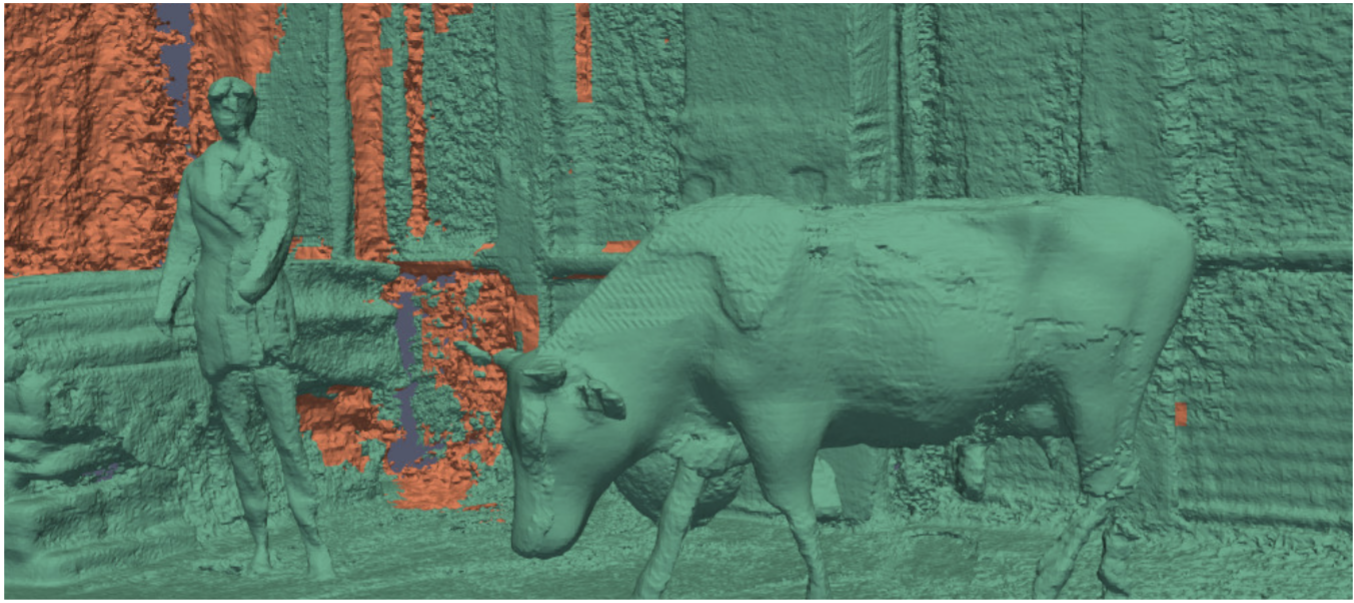
\includegraphics[width=0.8\textwidth]{super}
    \caption{Modèle 3D de l'environnement obtenu}
    \label{fig:super}
\end{figure}
\FloatBarrier


\subsection{Conclusion}


Le LiDAR permet une très grande précision qui peut même être améliorée avec la variation ou la modulation des longueurs d'ondes. Cependant, cette précision est étroitement liée à la nature de l'objet. En effet, les objets de couleur foncée réfléchissant moins les ondes électromagnétiques et les niveaux de bruits, entraîne une précision accrue. De la même manière, en fonction de la longueur d'onde, les sujets transparents ou à effet miroirs rendent donc la modélisation pratiquement impossible.
Dans le cas de la photogrammétrie, la précision est encore plus susceptible de varier. En effet, en fonction du type d'utilisation (de la photographie aérienne aux sujets d'échelle humaine) la résolution varie. En effet, comme cette méthode repose sur l'analyse de photographies, l'algorithme de traitement ainsi que la qualité des photos influent grandement sur le résultat final. De plus, on retrouve les mêmes problèmes qu'avec le LiDAR c'est-à-dire avec les faibles contrastes et objets transparents.





%%%%%%%%%%%%%%%%%%%%%%%%%%%%%%%%%%%%%%%%%%%%%%%%%%%%%%%%%%%%%
%% METHODES DE STOCKAGE
%%%%%%%%%%%%%%%%%%%%%%%%%%%%%%%%%%%%%%%%%%%%%%%%%%%%%%%%%%%%%
\section{Méthodes de stockage}

\subsection{Maillages 3D}
Nous commenceront par le cas des maillages 3D car plus simple à décrire. Il faut pour ce faire représenter les liens entre chaque vertex. Il existe une multitude de formats avec quelques variantes, nous nous concentreront ici sur le format gTIFF. Ce nouveau format compte permettre l'apparition de la 3D sur le web. Il faut pour décrire un mesh 3D l'ensemble de ses vertexes, avec leur position dans l'espace ainsi que la matrice des faces du mesh, qui en fonction du mode de rendu souhaité, peut contenir les adresses des 3 ou 4 sommets qui la compose. En fonction des formats on peut aussi ajouter d'autres informations relatives à chaque face du modèle, comme la texture, la couleur, la normale associé (ou pointe de la face)... 
Le stockage, la lecture, la compression et le traitement des maillages 3D sont donc facilités par toutes ces informations qu'on peut associer.

\subsection{Nuages de points}
Le cas des nuages de points est beaucoup plus complexe. En effet la seule information dont on dispose ici est la liste de points, avec des informations uniquement liées aux points eux même; aucune information liant les points entre eux n'est disponible. Les formats les plus classiques sont donc uniquement une liste de points avec leur informations spatiales et les caractéristiques supplémentaires (couleur, normale...). Mais les possibilités de traitement se voient limités (ce que l'on retrouve lorsque nous parlerons de l'utilisation des maillages et des nuages de points). On se trouve confronté à un problème simple en apparence qui se révèle complexe lorsque le nombre de points augmente : trouver les voisins d'un point. En effet bien que ce soit une étape essentielle pour tout traitement sur les nuages de points, elle peut s'avérer très difficile.

\subsubsection{K-nearest neighbour}
 L'un des problème le plus fréquent : comment trouver les k points voisins (appartenant à $P$) les plus proches du point considéré $y_{0}$ :
 
 $$ N_{KNN}(y_{0}, P, k) = \{x_{i} \in P | \|y_{0} - x_{i}\| \leq \|y_{0} - x_{i+1} \|, i<k\} $$
 
 
la complexité de ce problème, sans changer notre vision du nuage de points, évolue de manière exponentielle par rapport à la taille du nuage de points. On est alors dans l'incapacité de résoudre ce problème pour de grands nuages de points.
\newline
Il a alors été mis en place des structures plus optimisées de représentation et de stockage du nuages de points pour permettre leur traitement :

\subsubsection{Grilles}
\begin{wrapfigure}{r}{0.5\textwidth}
  \begin{center}
    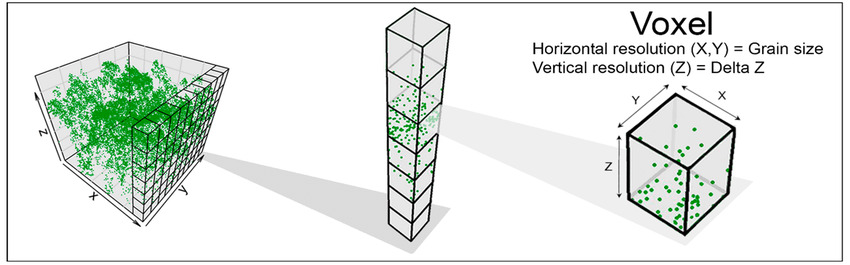
\includegraphics[width=0.48\textwidth]{voxel}
  \end{center}
  \caption{Grille volumétrique}
\end{wrapfigure}
Les grilles volumétriques sont les structures les plus basiques utilisées pour accélérer le traitement des nuages de points (surtout pour les problèmes de voisins). Elles consistent en une répartition de l'espace en de petits cube 3D appelés voxels. Nous allons alors assigner les points situés dans chaque voxel. Puis lorsque nous voudrons calculer leurs voisins on travaillera uniquement avec les points associés au voxel où se trouve notre point.


\subsubsection{Octrees}

\begin{wrapfigure}{r}{0.2\textwidth}
  \begin{center}
    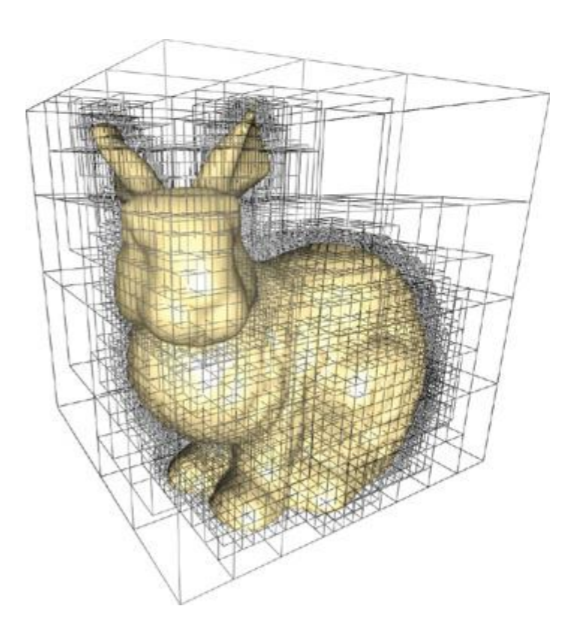
\includegraphics[width=0.3\textwidth]{octree}
  \end{center}
  \caption{Octree Représentation}
\end{wrapfigure}

Représentation assez similaire aux grilles volumétriques, les octrees développent le principe en ajoutant une composante : On partitionne toujours l'espace en voxels, mais on utilise un arbre hiérarchique à la place d'une grille simple. La racine de l'arbre correspond à un cube qui contient tout le nuage de points. Puis ce cube est divisé en sous cubes deux fois plus petits que le cube d'origine. On répète cette étape récursivement jusqu'à une taille minimale définie. Les cubes les plus petits sont donc les feuilles de notre arbre. lorsque l'on essaye de résoudre le problème KNN on part alors des feuilles et on remonte dans la zone autour du point de travail.
\newline
Cette représentation est particulièrement adaptée pour les nuages de points de forme géométrique. Elle a la particularité de consommer peu de mémoire et d'être particulièrement efficace. C'est pour ces raisons que cette méthode est très utilisée dans le cadre de nuages de points très grands. Mais la principale limitation des Octree est leur optimisation : pour les espace euclidiens 3D, si l'on augmente la dimension de l'espace ils perdent en efficacité.

\subsubsection{KdTrees}
Dernière représentation possible, les Kd-Tree. Ils peuvent être considérés comme une généralisation des octrees à toutes les dimensions. Ils partionnent eux aussi l'espace, mais cette fois ci chaque demi-espace est défini à l'aide d'hyperplans.


%%%%%%%%%%%%%%%%%%%%%%%%%%%%%%%%%%%%%%%%%%%%%%%%%%%%%%%%%%%%%
%% DOMAINES D'APPLICATION
%%%%%%%%%%%%%%%%%%%%%%%%%%%%%%%%%%%%%%%%%%%%%%%%%%%%%%%%%%%%%
\section{Domaines d'applications et utilisation}
Dans cette section nous étudierons les différents domaines d'application relatifs aux deux méthodes.

\subsection{Maillages 3D}
Il vient tout d'abord de présenter le cas des maillages 3D. En effet, dans la pratique ce sont eux que l'on utilise le plus. Nous allons retrouver leur utilisation dans tous les domaines visuels (Jeux vidéos, simulation 3D), mais aussi scientifique (Simulation numérique, analyse...) tout comme dans l'ingénierie (CAO, simulation physique...).
\subsubsection{Rendu 3D}
L' utilisation massive des maillages 3D peut s'expliquer par leurs propriétés. En effet pour permettre le rendu 3D et afficher à l'écran une image des modèles 3D les GPU (les cartes graphiques) ont besoin des informations géométrique du maillage 3D (les triangles, les liens entres chaque vertex). De même pour coloriser ou texturer nos mesh 3D, il faut avoir un système de coordonnées sur le modèle 3D pour ensuite projeter la texture. Les programmes qui sont ensuite exécutés sur la carte graphique sont capables (et optimisé) afin de réaliser ce type d'opérations, mais demandent également des primitives géométrique sous forme de vertexes et de triangles.

Il existe plusieurs types de rendu (Forward rendering ou Deferred Rendering) ,mais leurs présentations dépassent le cadre de ce rapport. Nous présenterons ici une version simple mais universelle d'un rendu 3D pour montrer l'importance de la structure des maillages 3D :

\begin{figure}[h]
    \centering
    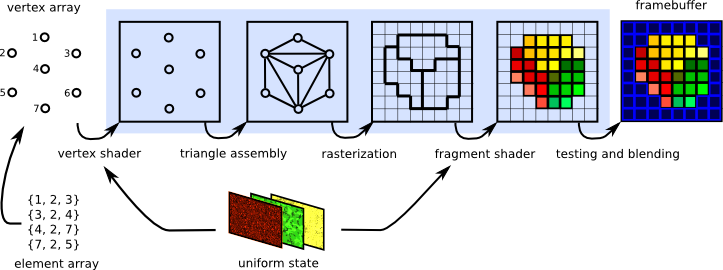
\includegraphics[width=0.8\textwidth]{gpuWorkflow}
    \caption{Etapes de rendu}
    \label{fig:render}
\end{figure}
\FloatBarrier

\newpage

Avec la complexité des moteurs de rendu aujourd'hui nous arrivons à faire des rendus de très bonne qualité :

\begin{figure}[h]
    \centering
    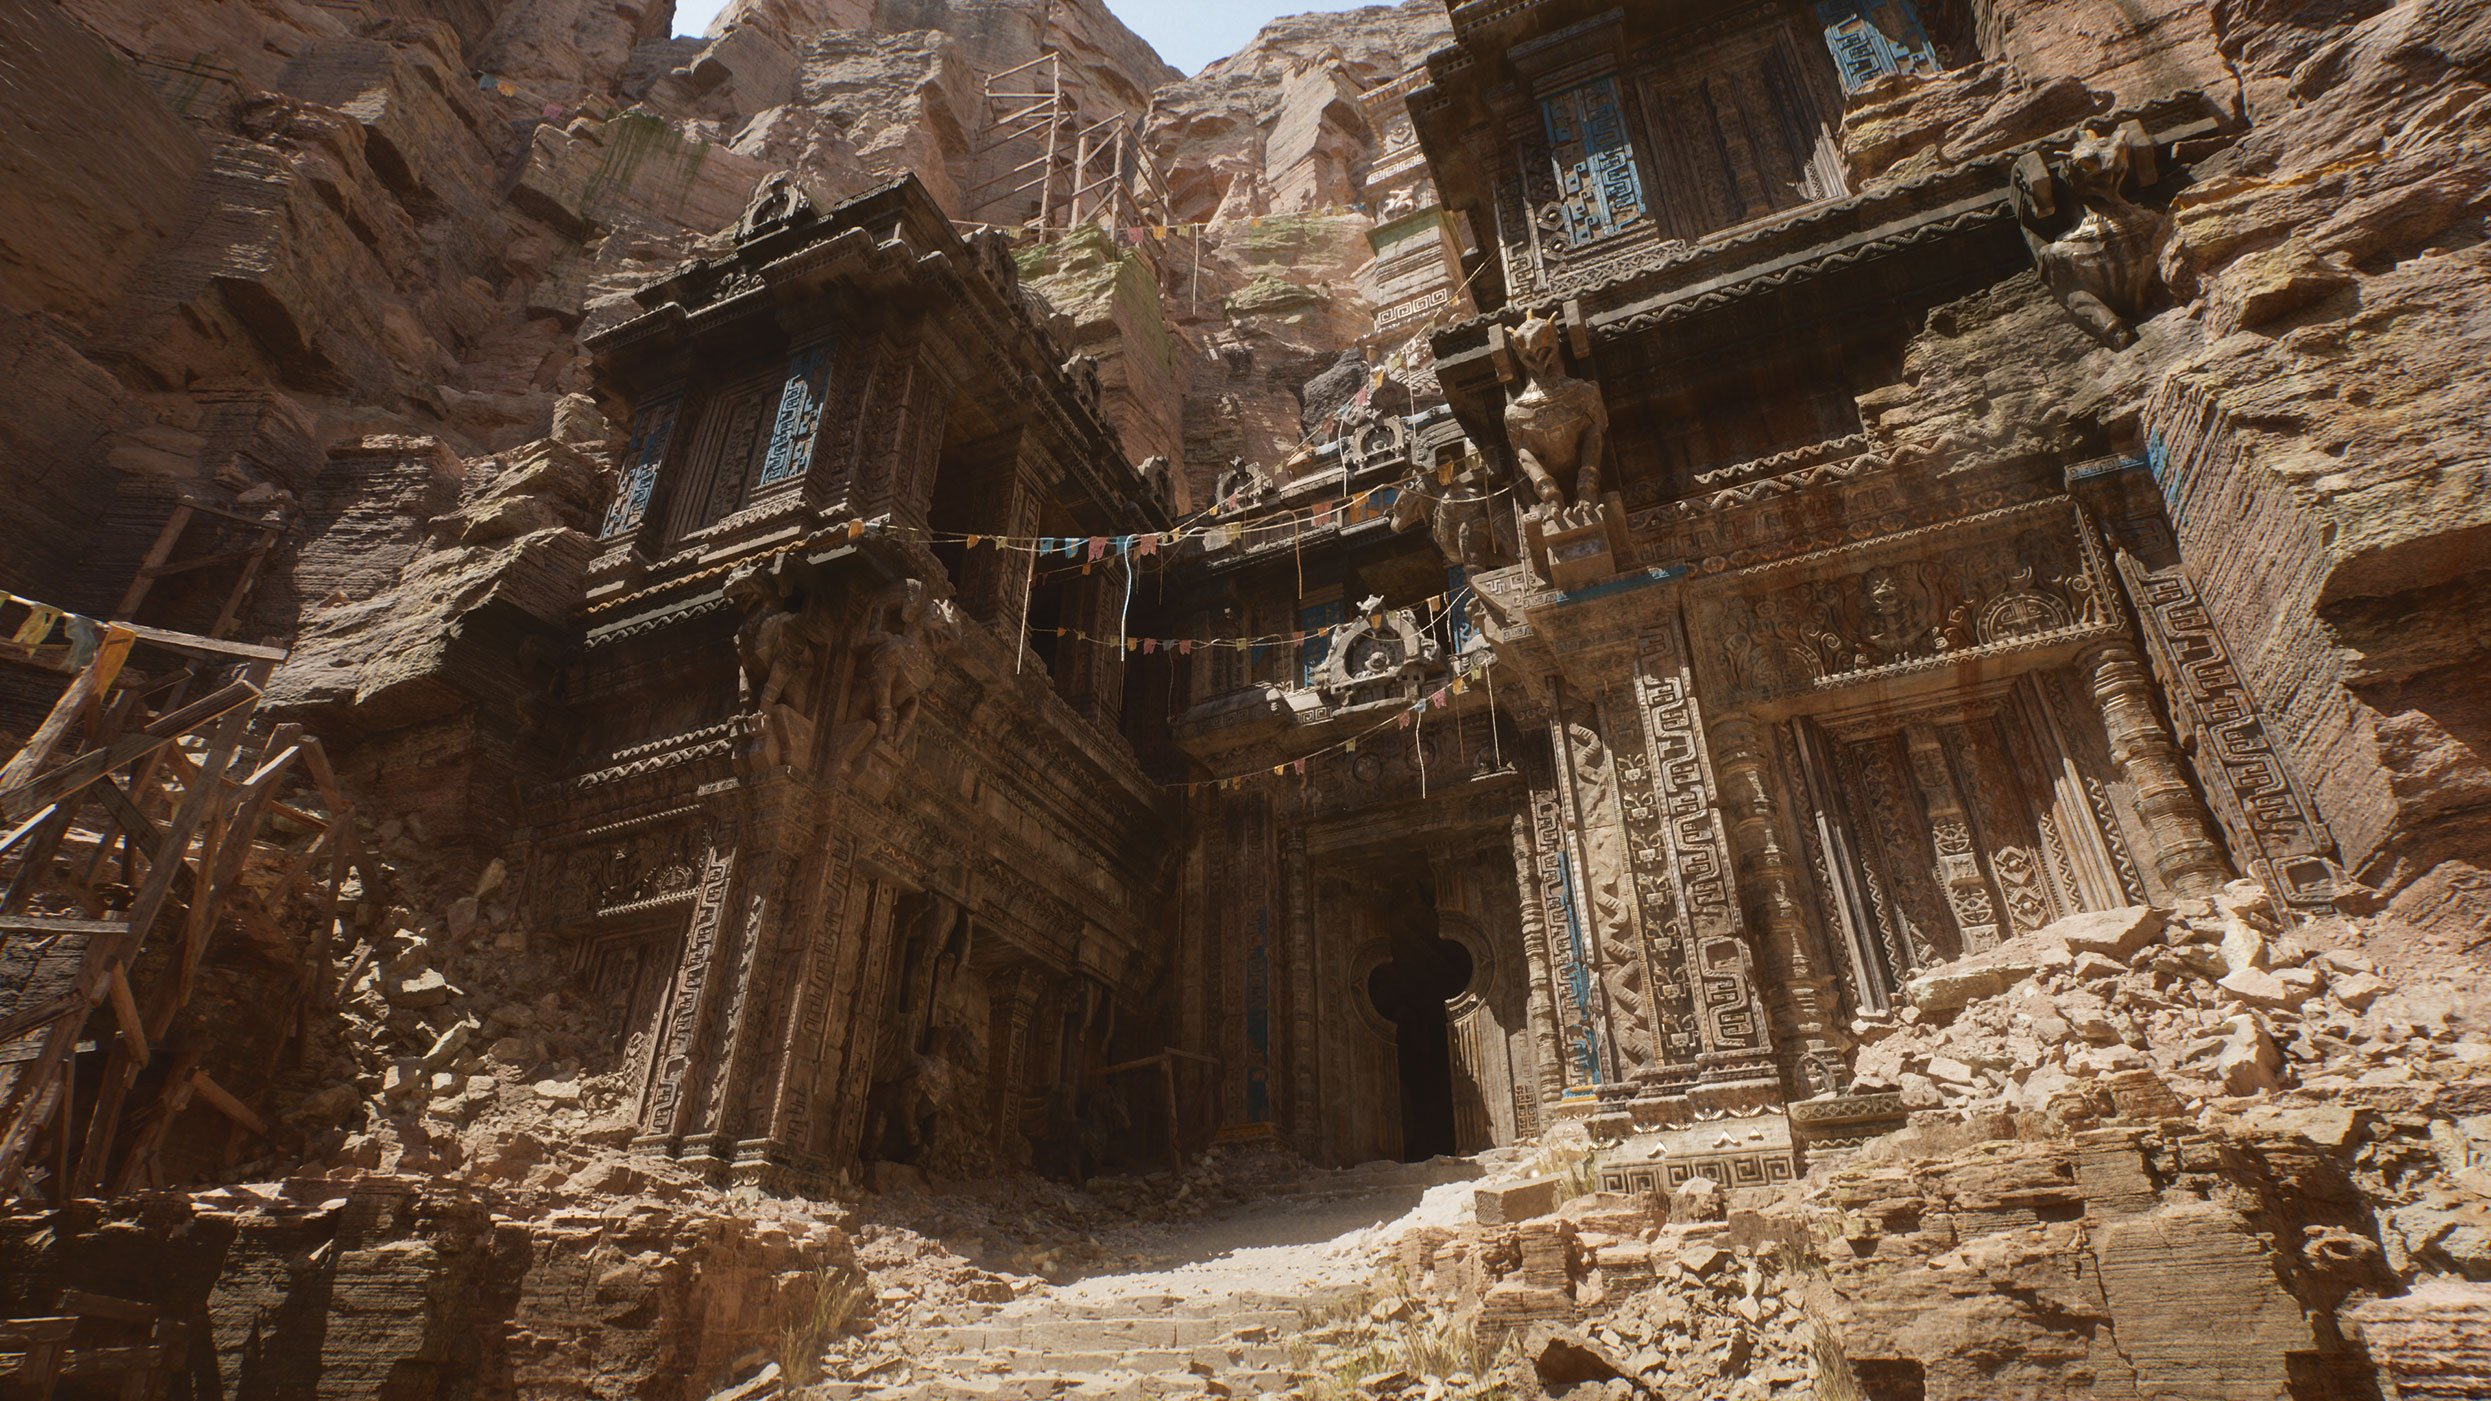
\includegraphics[width=0.8\textwidth]{ue5}
    \caption{Exemple de rendu du moteur Unreal Engine 5, avec les technologie Nanite (virtualisation des maillages 3D) et Lumen (Real time global illumination)}
    \label{fig:render}
\end{figure}
\FloatBarrier


\subsubsection{Ingénierie}
Dans le domaine de la CAO et de la simulation pour l'Ingénierie, les maillages 3D jouent un rôle central. En effet les ingénieurs ont besoin de connaître la topologie des objets sur lesquels ils travaillent. De même pour la simulation de déformation des pièces ou la simulation de fluides :

\begin{figure}[h]
    \centering
    \subfloat[ Logiciel de CAO CATIA]{{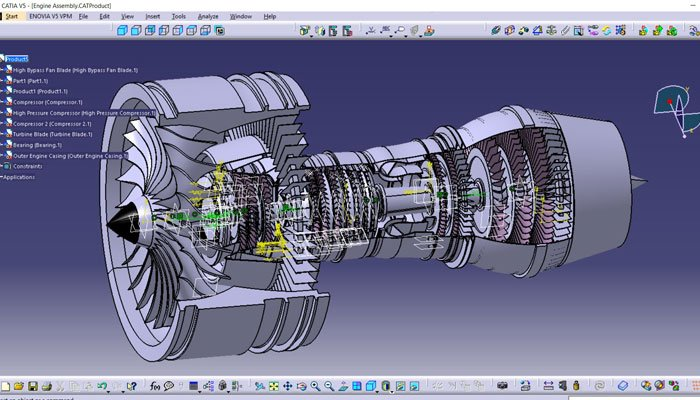
\includegraphics[width=6cm]{CATIA} }}
    \qquad
    \subfloat[ Simulation flux de l'air CATIA]{{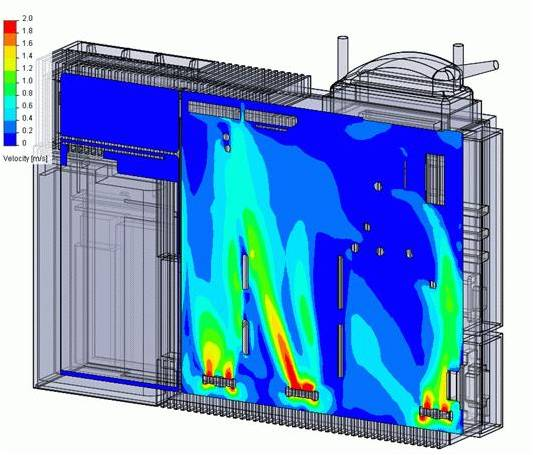
\includegraphics[width=5cm]{sim} }}
    \caption{Différentes utilisations des maillages 3D en CAO}
    \label{fig:CATIA}
\end{figure}
\FloatBarrier

Ces deux partie font office d'exemple, les maillages 3D ont de nombreux autres domaines d'application. Cependant, la nécessité d'utiliser pour obtenir des rendus 3D leurs, favorise l'utilisation de mesh 3D dans de nombreux cas.


\subsection{Nuages de points}
Les nuages de points étant moins riches au niveau de l'information qu'ils portent, cela les rend moins complexe à traiter. En effet, il n'y a pas besoin de considérer leurs topologies. Ils sont aussi, comme nous avons pu le voir dans le chapitre sur les méthodes d'acquisition, un type de données brutes facile à obtenir. Nous allons voir quelques domaines d'application représentatifs.

\subsubsection{Robotique et drones}
Dans le cadre de la robotique les nuages de points jouent un rôle central. Souvent équipé de capteur laser type LiDAR, le robot à donc accès en temps réel à sont environnement proche sous forme de nuages de points. C'est donc cette représentation qui sera utilisée pour faire les traitements les plus critiques (qui doivent être fait en temps réel), on peut notamment citer :
\begin{itemize}
    \item Analyse de l'environnement
    \item Détection
\end{itemize}
Nous pouvons donner comme exemple : la voiture autonome où la détection des personnes et autres voitures se fait au niveau du nuages de points :

\begin{figure}[h]
    \centering
    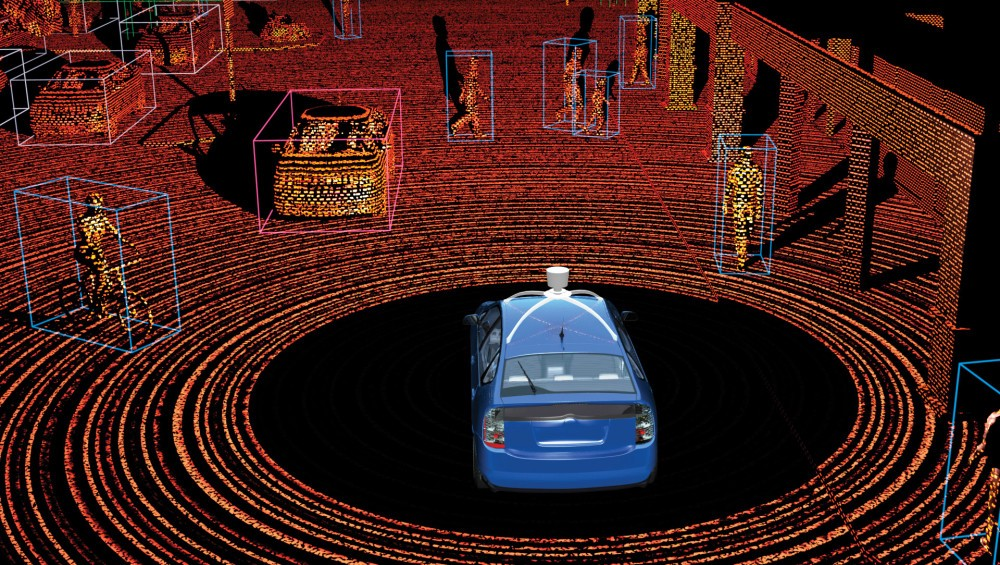
\includegraphics[width=0.8\textwidth]{car}
    \caption{Voiture autonome avec LiDAR, détection des voitures et piétons}
    \label{fig:car}
\end{figure}
\FloatBarrier

\newpage
Même si les nuages de points permettent une analyse de l'environnement du robot, il est souvent aussi nécessaire d'obtenir une version en maillage 3D afin de faire par exemple du path planning. Pour ce faire dans la majorité des cas c'est à partir du nuage de points que l'on générera un mesh 3D.

\begin{figure}[h]
    \centering
    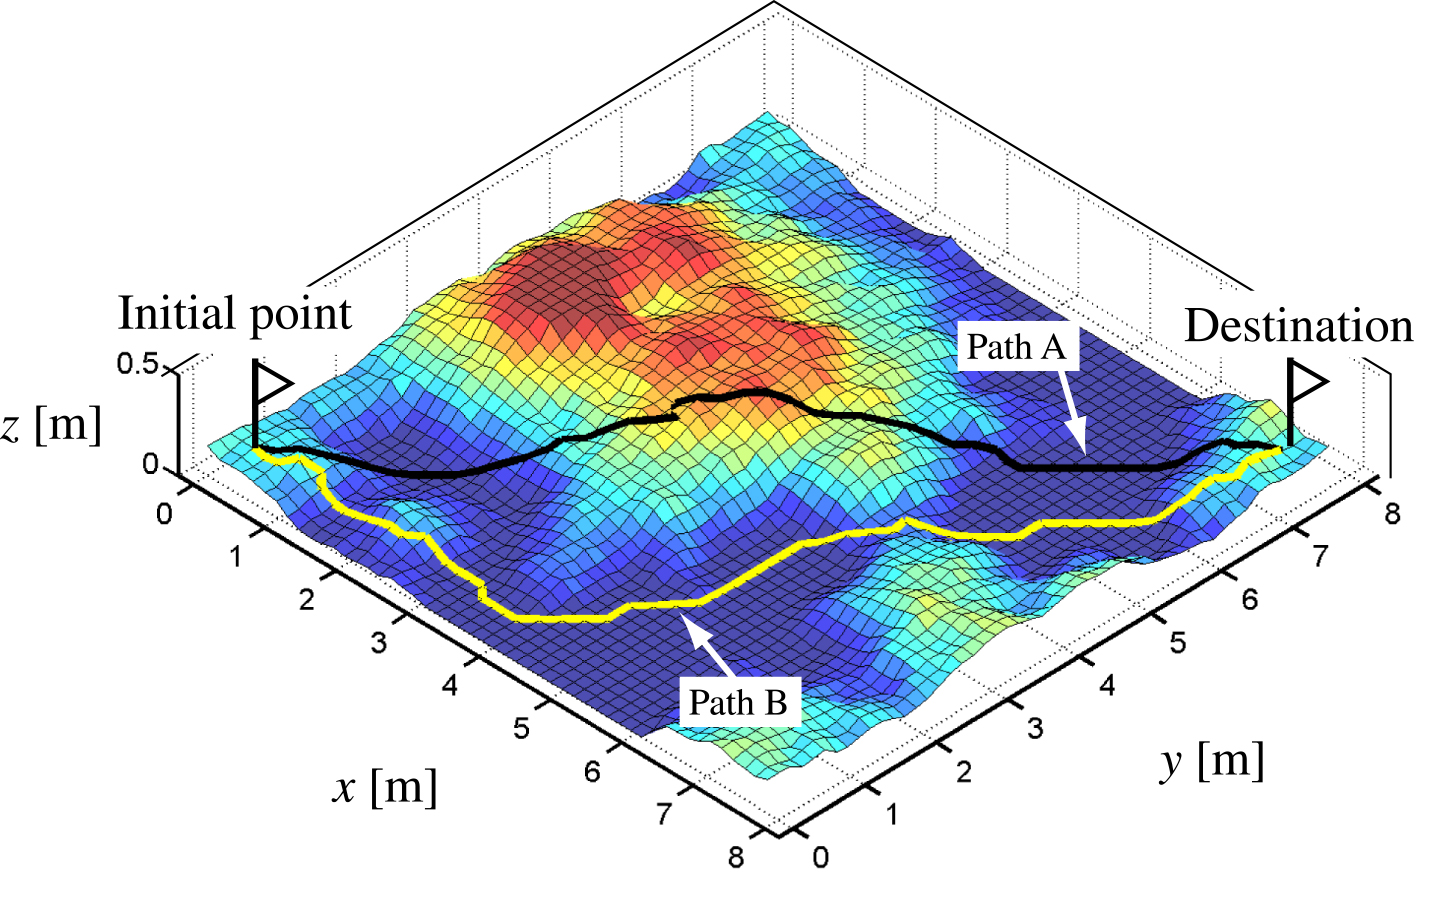
\includegraphics[width=0.5\textwidth]{path}
    \caption{Vertion en maillage 3D du sol d'un environnement pour du path planning}
    \label{fig:Path}
\end{figure}
\FloatBarrier

\subsubsection{Topographie}
L'acquisition simple des nuages de points par LiDAR ou photogrammétrie permet des collectes topographiques par avion ou par capteur au sol simple. Puis, après traitement, on obtient des cartes 3D sous forme de nuages de points. Il est alors possible de les convertir sous forme de maillages 3D, pour faciliter le rendu et l'affichage.

\begin{figure}[h]
    \centering
    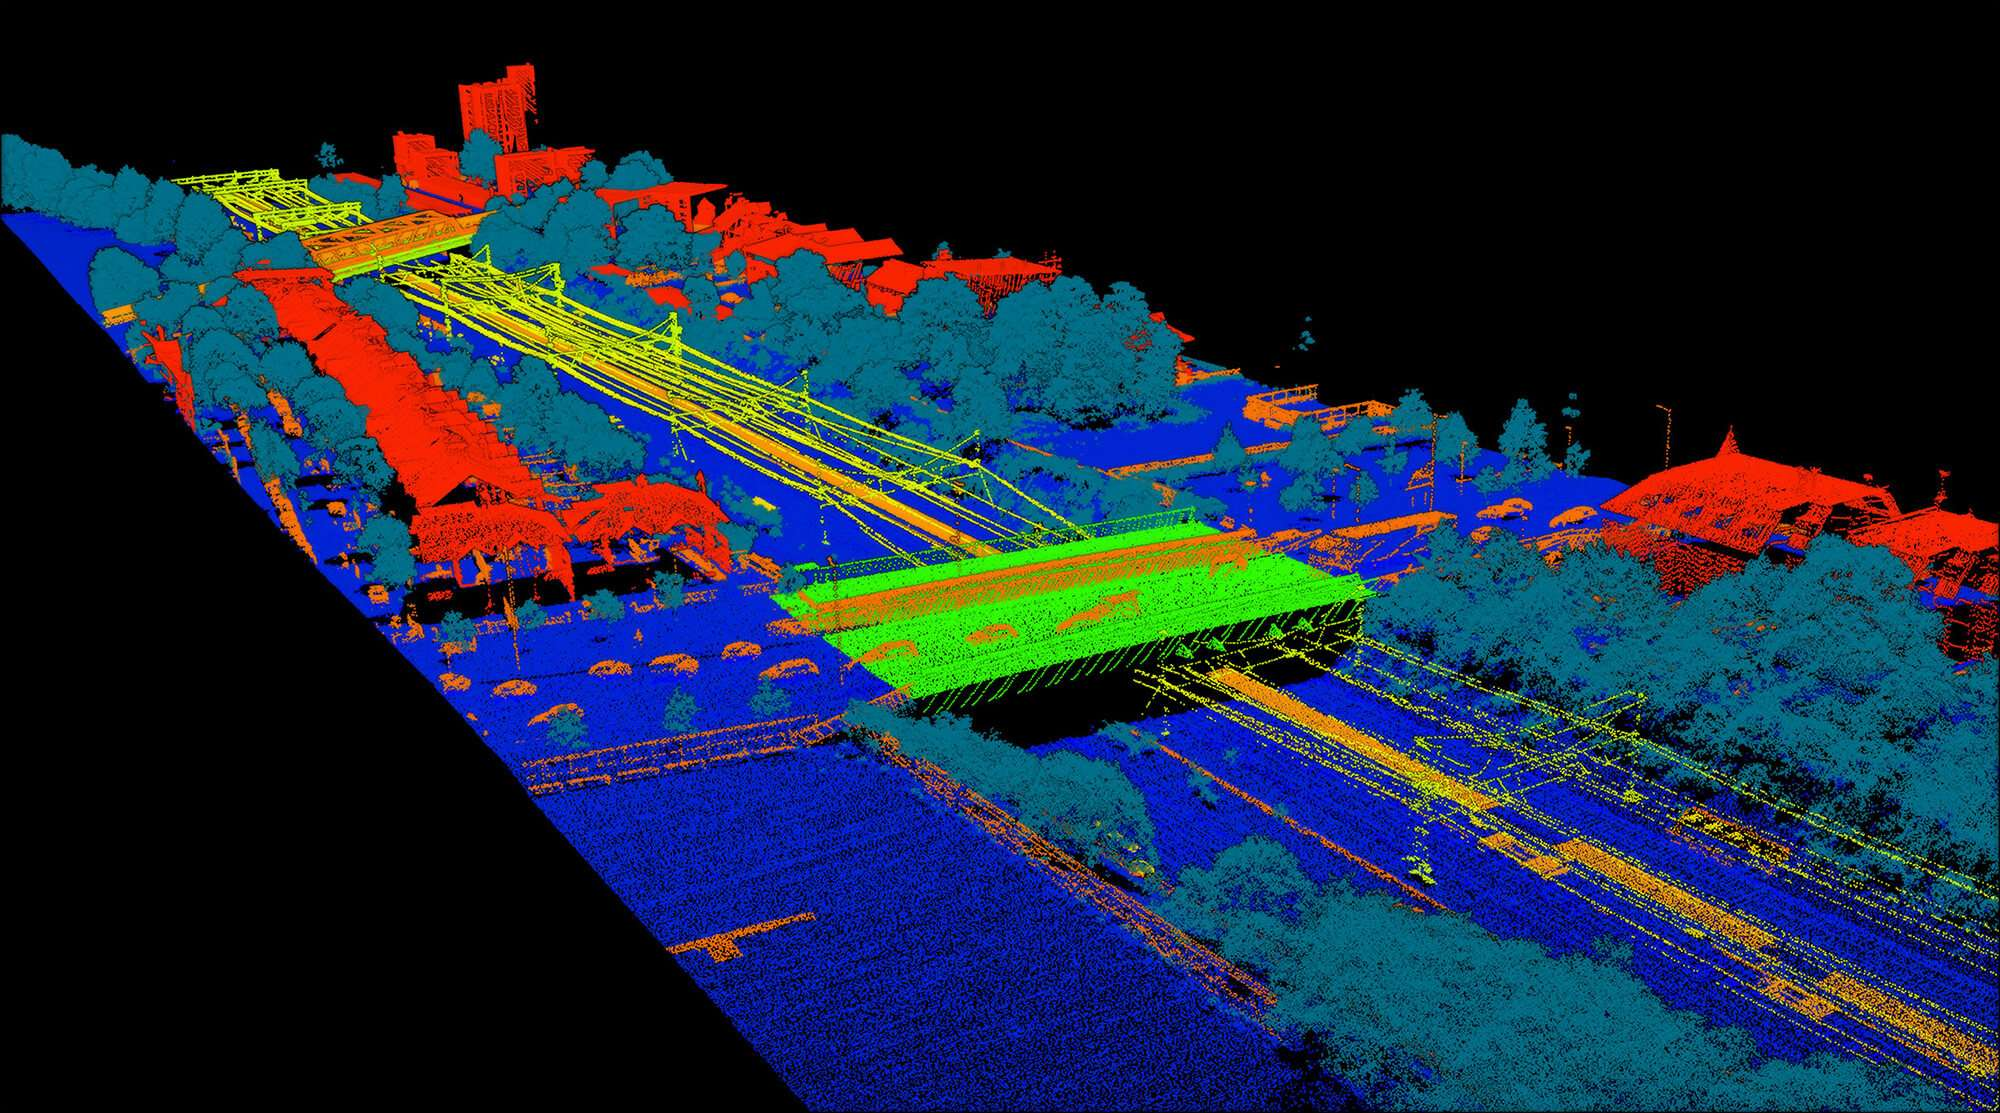
\includegraphics[width=0.65\textwidth]{map}
    \caption{Nuages de points après collecte}
    \label{fig:map}
\end{figure}
\FloatBarrier

\newpage

Lorsque l'on parle de relevé topographique, il est possible de générer plusieurs types d'informations sous forme de maillages 3D :
\begin{itemize}
    \item DSM (Digital Surface Elevation)
    \item DEM (Digital Elevation Model)
    \item DTM (Digital Terrain Model)
\end{itemize}

\begin{figure}[h]
    \centering
    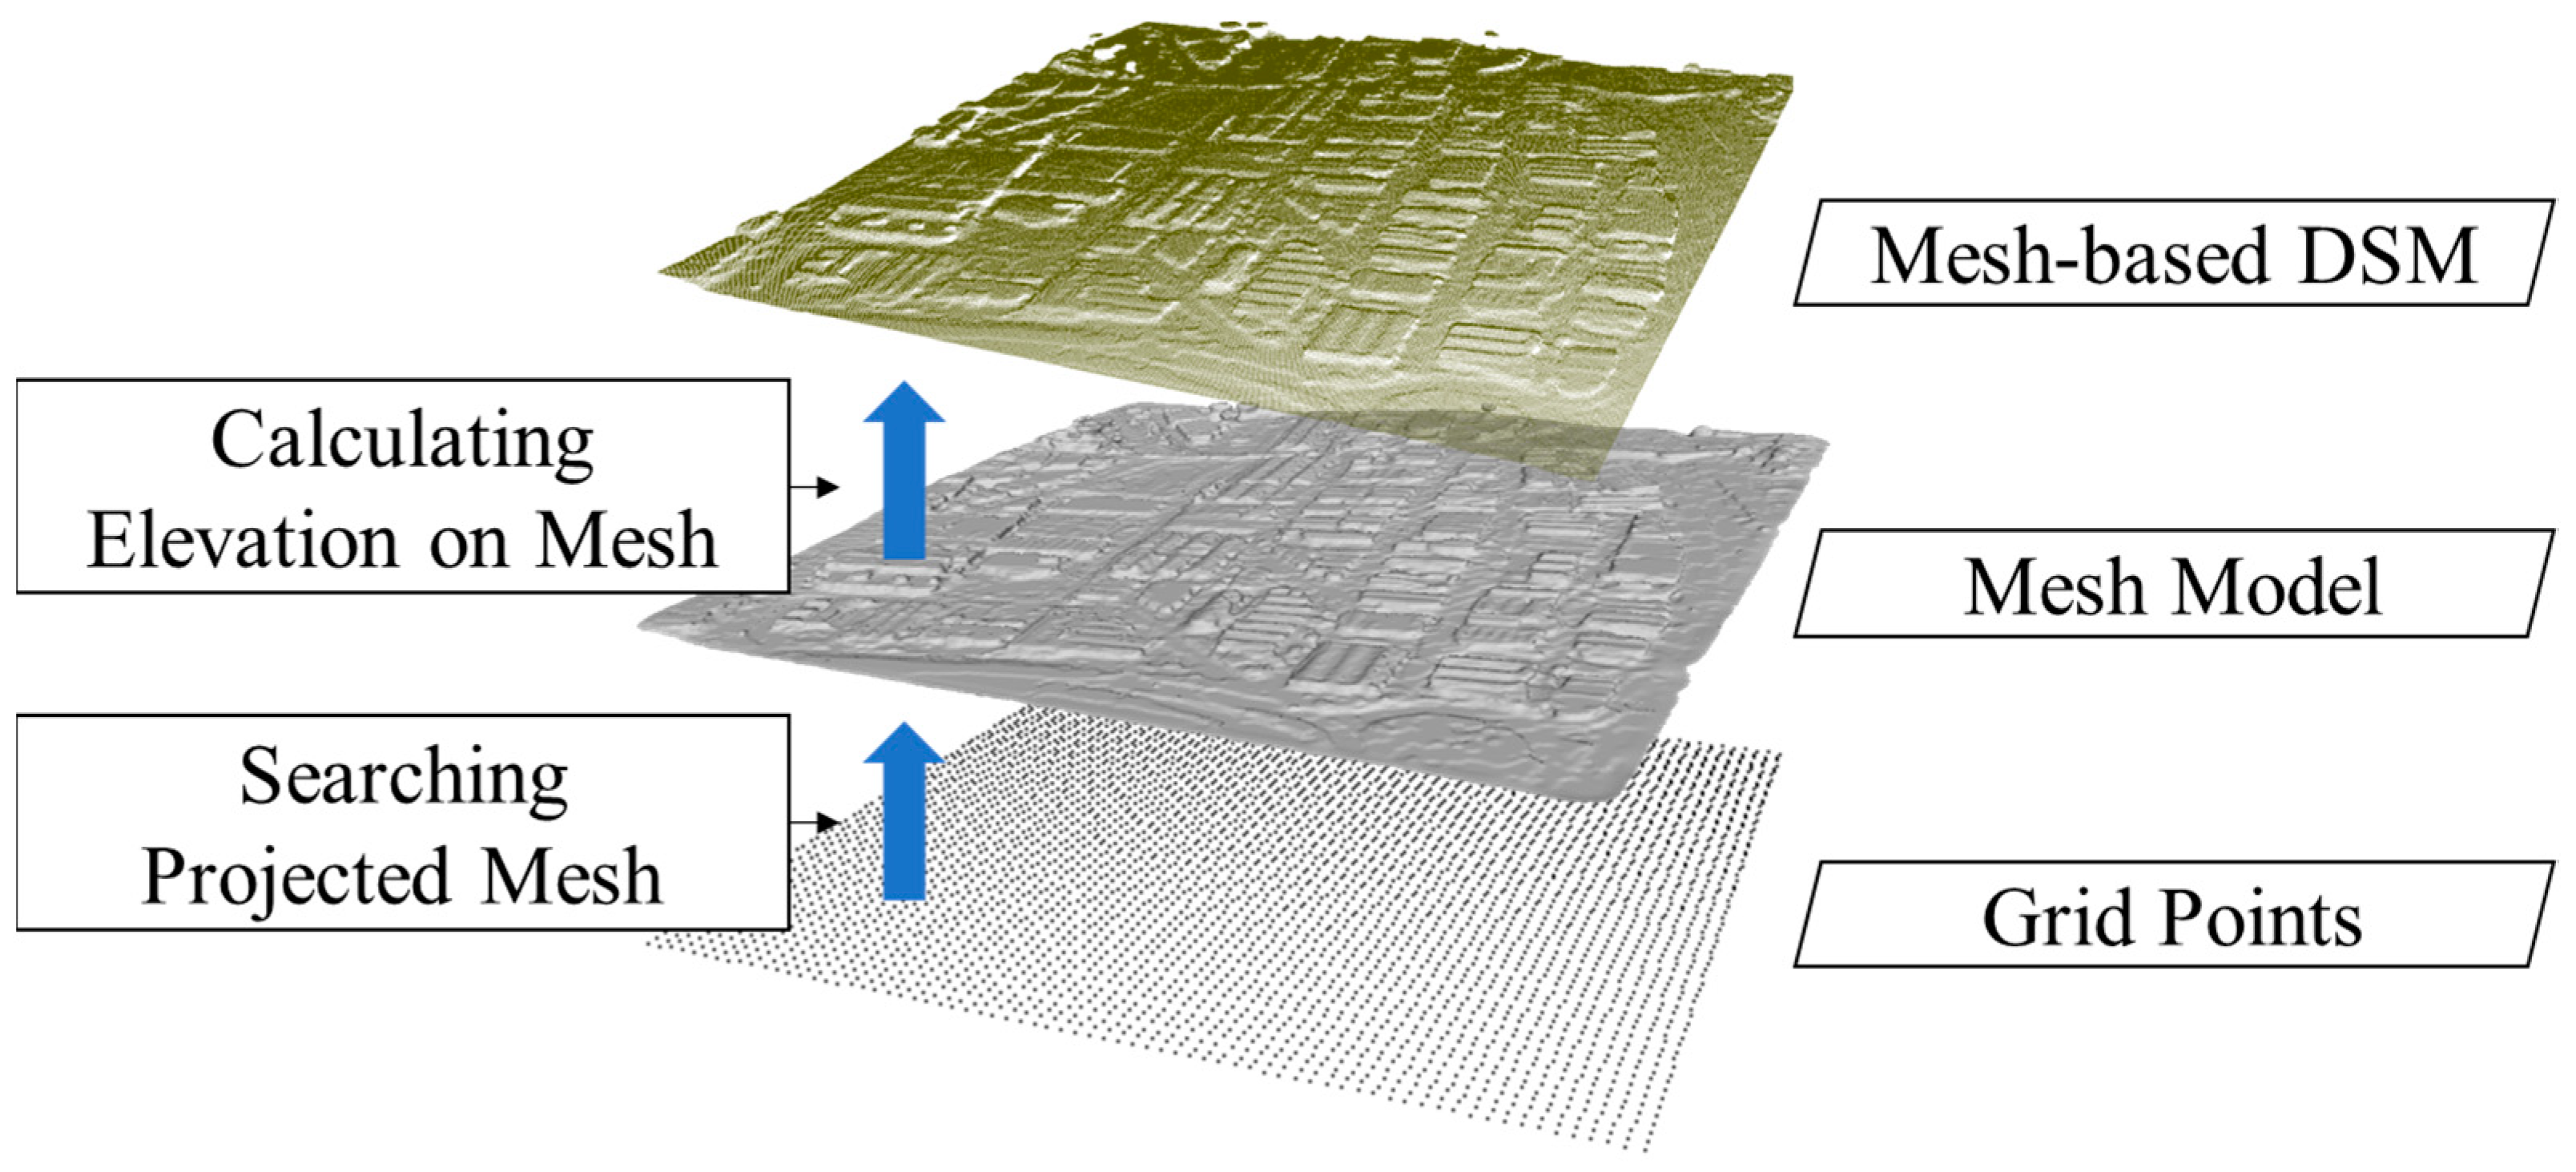
\includegraphics[width=0.8\textwidth]{process}
    \caption{Transition entre nuages de points et maillages 3D}
    \label{fig:car}
\end{figure}
\FloatBarrier


Les nuages de points sont donc souvent utilisés comme moyen de transition. Faciles à obtenir, ils permettent une analyse de l'environnement, mais sont surtout utilisés comme moyen transitoire pour obtenir un maillage 3D de l'environnement qui permet un rendu 3D et un traitement plus poussé (path planning, occupency grid...).


%%%%%%%%%%%%%%%%%%%%%%%%%%%%%%%%%%%%%%%%%%%%%%%%%%%%%%%%%%%%%
%% CONCLUSION
%%%%%%%%%%%%%%%%%%%%%%%%%%%%%%%%%%%%%%%%%%%%%%%%%%%%%%%%%%%%%
\section{Conclusion}
\paragraph{•} Pour conclure, le Séminaire : Image et Multimédia et Application, nous a permis de découvrir deux technologies de numérisation et de visualisation 3D : nuage et maillage de points. En particulier, les enseignements suivis nous ont permis de comprendre les spécificités et similitudes de ces deux méthodes, et donc de réaliser une étude comparative.

\paragraph{•} Tout d'abord, bien que les nuages et les maillages de points ont le même objectif (permettre de représenter fidèlement des éléments en 3D dans l'espace), la première disparité entre ces deux méthodes est leurs définitions et propriétés. En effet, un nuage de points est définit comme une liste de coordonnées non-reliées et non-ordonnées d'un espace en 3D. Tandis qu'un maillage de points fait communément référence à une liste de points précisément ordonnés et géométriquement reliés. Par conséquent, la complexité supérieure de la définition et des propriétés des maillages de points permet de fournir plus d'informations que les nuages de points.

\paragraph{•} Or, puisque les maillages de points fournissent davantage d'informations, construire un maillage de points nécessite des méthodes plus complexes. En effet, son acquisition nécessite une lecture continue de l'espace 3D. C'est pourquoi, la méthode souvent privilégiée pour la construction d'un maillage de points est une méthode hybride consistant à construire un mesh à partir d'un nuage de points (qui est plus facile à établir) comme l'Advancing Front Surface Reconstruction. Toutefois des méthodes d'acquisition telles que l'utilisation de scanner IRM ou utilisant une intelligence artificielle permettent de construire un maillage de point directement. De même, les technologies de Lidar permettent de construire des nuages de points directement. En particulier, la démocratisation des Lidar et leur coût de plus en plus abordable pour les startups, mais également pour les particuliers, pourraient permettre une utilisation de plus en plus importante des nuages 3D, et des méthodes hybrides pour obtenir des mesh 3D, bien plus coûteux à construire directement.

\paragraph{•} Par ailleurs, ces différences de définition et d'acquisition impliquent également des disparités concernant le stockage des données. En effet, la quantité plus importante d'informations fournies par les mesh permet de faciliter le stockage, la lecture, la compression et le traitement des maillages 3D. Au contraire, puisque seules quelques caractéristiques et le positionnement des points sont stockés dans un nuage de points, les possibilités de traitement sont alors réduites. En particulier, déterminer les points voisins d'un autre est difficile avec un nuage de point, contrairement au cas des mesh puisque les points sont reliés et ordonnés par l'intermédiaire de formes géométriques.

\paragraph{•} Enfin, toutes ces spécificités impliquent des champs d'application différents. En effet, les maillages 3D sont souvent utilisés  pour améliorer l'affichage graphique de modèles 3D sur un écran, ainsi que pour mieux représenter la topologie des objets en ingénierie. D'un autre côté, les nuages de points sont davantage utilisés pour des situations et projets ne nécessitant pas une précision accrue, mais plutôt une vitesse de traitement rapide notamment en robotique et pour l'usage de drones.

